\documentclass[11pt]{article}
\usepackage[letterpaper, left=.8in, top=0.9in, right=.8in, bottom=0.70in,nohead,includefoot, verbose, ignoremp]{geometry}
%\usepackage{charter} %choose default font ... your choice here % {mathptmx} % mathrsfs} % mathptmx} %mathpple} %mathpazo}
\usepackage[round]{natbib}
\usepackage{enumerate} % for different labels in numbered lists 
%\usepackage{xy}\xyoption{all} \xyoption{poly} \xyoption{knot}  
\usepackage{latexsym,amssymb,amsmath,amsfonts,graphicx,color,amsthm,enumerate,natbib,mathtools, bm, float} %,fancyvrb,movie15
\usepackage{dsfont}
\usepackage[pdftex,pagebackref=true]{hyperref}
\usepackage[svgnames,dvipsnames,x11names]{xcolor}
\hypersetup{
colorlinks,%
linkcolor=RoyalBlue2,  % colour of links to eqns, tables, sections, etc
urlcolor=Sienna4,   % colour of unboxed URLs
citecolor=RoyalBlue2  % colour of citations linked in text
}
\pagestyle{empty} % no page number on front page
\usepackage{todonotes}
%\usepackage{mathrsfs} % For \mathscr function

%\renewcommand{\includegraphics}{}  % use this to suppress inclusion of figs for proofing

% custom definitions ...
\def\eq#1{equation (\ref{#1})}
\def\pdf{p.d.f.\ } \def\cdf{c.d.f.\ }
\def\pdfs{p.d.f.s} \def\cdfs{c.d.f.s}
\def\mgf{m.g.f.\ } \def\mgfs{m.g.f.s\ }
\def\ci{\perp\!\!\!\perp}                        % conditional independence symbol
\def\beginmat{ \left( \begin{array} }
\def\endmat{ \end{array} \right) }
\def\diag{{\rm diag}}
\def\log{{\rm log}}
\def\tr{{\rm tr}}
\def\etr{{\rm etr}}
\def\Ei{{\rm Ei}}
\def\cD{\mathcal{D}}
\def\cS{\mathcal{S}}
\def\cM{\mathcal{M}}
%\newtheorem{thm}{Theorem}
\newcommand{\Reals}{\mathbb R}
\newcommand{\Beta}{\mathrm{Beta}}
\newcommand{\KL}{\mathrm{D}_{KL}}
\newtheorem{thm}{Theorem}[section]
\newtheorem{lemma}{Lemma}[section]
\newtheorem{cor}{Corollary}[section]
\newcommand{\df}{\vcentcolon=}
\newcommand{\ex}{{\mathbb E}}
\newcommand{\pfrac}[2]{\left(\frac{#1}{#2}\right)}

\DeclareBoldMathCommand{\balpha}{\alpha}
\DeclareBoldMathCommand{\bbeta}{\beta}
\DeclareBoldMathCommand{\btheta}{\theta}
\DeclareBoldMathCommand{\bS}{S}
\DeclareBoldMathCommand{\bx}{x}
\DeclareBoldMathCommand{\bw}{w}
\DeclareBoldMathCommand{\bv}{v}
%

%%My Definitions
\def\qed{\hfill $\square$}
\newcommand{\indep}{\mathop{\perp\!\!\!\!\perp}}

\def\ts{\tilde{s}}

%% Document starts here ...
%%
\begin{document}
\vspace{-1in}
\title{A Sequential Hypothesis Test for Implementation Errors and Missing Data in Simply Randomized Experiments with Applications to A/B Testing}
\author{\Large Michael Lindon \\ Optimizely \and \Large Alan Malek \\ Optimizely}
\maketitle 
%\centerline{{\color{RoyalBlue2}{Due: someday.}}}\bigskip
%\thispagestyle{empty}
\begin{abstract}
  Simply randomized designs are one of the most common controlled experiments used to study causal effects.
  Failure of the assignment mechanism, to provide proper randomization of units across treatments, or the data collection mechanism, when data is ``missing not at random'', can render subsequent analysis invalid if not properly identified.
In this paper we demonstrate that such practical implementation errors can often be identified, fortunately, through consideration of the total unit counts resulting in each treatment group.
  Based on this observation, we introduce a sequential hypothesis test constructed from Bayesian multinomial-Dirichlet families for detecting practical implementation errors in simply randomized experiments.
By establishing a Martingale property of the posterior odds under the null hypothesis, frequentist Type-I error is controlled under both optional stopping and continuation via maximal inequalities, preventing practitioners from potentially inflating false positive probabilities through continuous monitoring.
  In contrast to other statistical tests which are performed once all data collection is completed, the proposed test is sequential - frequently rejecting the null during the process of data collection itself, saving further units from entering an improperly-executed experiment.
  We illustrate the utility of this test in the context of online controlled experiments (OCEs), where assignment is automated through code and data collected through complex processing pipelines, often in the presence of unintended bugs and logical errors.
Confidence sequences posessing nominal sequential frequentist coverage probabilities are provided and their connection to the Bayesian support interval is examined.
The differences between the pure Bayesian and sequential frequentist testing procedures are finally discussed through a conditional frequentist testing perspective.
 
\end{abstract}


\section{Introduction}
\label{sec:intro}
Randomized treatment assignment satisfies many purposes in controlled experiments (see \cite{kempthorne}, \cite{cox} and \cite{rubin}).
Arguably the least controversial justfication is the attempt to remove any personal, systematic, or selection bias in the treatment assignment mechanism, although this is neither without criticism nor without alternative (see \cite{lindley} and \cite{kadane}).
Consider, for example, a medical researcher who administers a preferred experimental drug to only the patients most likely to recover.
Without explicitly conditioning on this information in the assignment mechanism, causal estimands such as the average treatment effect may be biased and overestimate the efficacy of the new drug (\cite{berry}).
Simply randomized experiments attempt to remove the possibility of bias by randomly assigning experimental units independently to treatment groups.
This design is useful in contexts where units enter the experiment sequentially, as opposed to all being simultaneously available like in completely randomized designs, and are often used in the technology industry to run online controlled experiments (OCEs) (\cite{oce}).
Formally, let there be $d$ treamtent groups, let $\triangle^d$ denote the $d$-dimensional simplex, let $\btheta_0 \in \triangle^d$ be a probability vector where element $\theta_{0,i}$ denotes the probability of any unit being assigned to treatment group $i$, and $\bx_j$ a random variable denoting the assignment outcome of the $j$th experimental unit.
We use boldface to emphasize vectors.
The simply randomized design can then be summarized by the following probabilistic assignment mechanism
\begin{equation}
  \label{eq:multinomialassignment}
  \bx_1,\bx_2, \dots \sim \text{Multinomial}(1,\btheta_0).
\end{equation}
The statistician may not be personally involved with the data collection process and may simply be told the assignment mechanism after being presented with the data for analysis.
The observant statistican has a right for concern, therefore, when they are provided with data which does not support the purported assignment mechanism.
For simply randomized experiments, the total unit counts assigned to each treatment group can provide evidence that the model \eqref{eq:multinomialassignment} is not true.
Indeed, this is a strong indicator that the experiment has not been conducted as expected; for example, the assignment mechanism could be biased, there could be systematic data loss, or generally when the data can be considered ``missing not at random'' (MNAR) \citep{missing-data}.
Such observations occurs frequently in OCEs and are colloquially referred to in the technology industry as \textit{sample ratio mismatches} (SRMs).

OCEs automate the assignment mechanism, data collection and data cleaning through code, which often introduces bugs and logical errors.
It is unsurprising, therefore, that \cite{fabijan} report that 6\% of all experiments performed in a at Microsoft contained bugs which were revealed by SRMs.
The authors describe in detail the engineering architecture required for assignment and data collection in OCEs and highlight how SRMs frequently reveal bugs therein.
They further provide a simple example of an experiment to study user engagement on an improved version of a web page is provided.
Not all visitors to a web page are human, however, and data must be cleaned to remove non-human interactions with the page, such as from web crawlers and scrapers.
Unfortunately the classification between human and non-human visitors is performed algorithmically, and some users in the treatment group were so engaged with the new page that they were accidentally classified as non-human and removed prior to the analysis - essentially removing units most in favour of the treatment, resulting in fewer units than expected being reported in the treatment group.
This is not an issue with the assignment mechanism, but in the data collection.
It is an example of a \textit{censoring} missing data mechanism, a special case of MNAR.

\cite{zhao} describe an example in which the user identifer becomes lost, preventing users from receiving a consistent experience over time, with some users initially assigned to the treatment becoming exposed to and recorded in the control - an example of noncompliance (\cite{imbens}).


Many other practical abnormalities can be revealed by considering the total counts in each treatment group after collection.
For this reason, industry practitioners now consider performing a post-experiment Chi-squared test against the null in equation \eqref{eq:multinomialassignment} best practice \citep{linkedin}; such a test will identify a SRM.
However, we note two deficiencies of this practice.
First, one only learns about a problem in the data after data collection has completed.
It is assumed that there is an implicit cost of including a unit in an experiment, and so ideally one would like to learn about such problems as soon as possible to prevent further units from entering an improperly executed-experiment.
Second, the desire to find SRMs early encourages practitioners to incorrectly \textit{continuously monitor} their experiments through the repeated application of significance tests without any multiplicity correction (\cite{armitage}).

In this paper, we propose a sequential test to identify SRMs that allows for optional stopping and optional continuation \todo{define optional stopping and continuation}.
Our method is inspired by Bayesian methods satisfying the \textit{stopping rule principle}, which requires that that statistical conclusions provided by a hypothesis test should be independent of the reason for stopping the experiment, which follows from the likelihood principle \citep{likelihood}.

The contributions of this paper focus, however, on obtaining frequentist properties of such a sequential test.
\todo{We should define what a sequential test is}
The paper is outlined as follows.
Section \ref{sec:srm_testing} defines a common Bayesian test through conjugate multinomial-Dirichlet models.
Section \ref{sec:theory} establishes the Martingale properties of the posterior odds under the null hypothesis, enabling a modified test to be developed which allows control of the frequentist Type-I error probabilities under both optional stopping and continuation.
This safely permits the online testing of hypothesis \eqref{eq:multinomialassignment} after every single observation, without inflating frequentist Type-I error, with the obvious advantage of being able to safely reject the null and discover a practical implementation error early in the beginning of an experiment - preventing experimental units being wasted on a faulty experiment.
Instance-specific upper-bounds on time-to-rejection are provided in terms of the KL divergence  between $\btheta_0$ and the actual generating distribution of the samples.
This sequential test is then inverted to define confidence sequences which possess nominal frequentist coverage probabilities.
Section \ref{sec:simulation} presents a number of simulation studies illustrating how false positive probabilities are dramatically inflated through the repeated significance testing using a Chi-squared test compared to the guarantees afforded by the proposed test.
We also study the number of samples needed to reject the null when the null is invalid.
The final section \ref{sec:discussion} connects these contributions with existing literature.
In particuar, the confidence sequence defined in Theorem~\ref{thm:confidence_sequence} is identified as the Bayesian support interval of \cite{support_interval} through an application of the Savage-Dickey density ratio.
The differences between the pure Bayesian test and the proposed test are discussed from the perspective of conditional frequentist testing \citep{conditional_frequentist_simple, conditional_frequentist_precise, conditional_frequentist_composite}.





\section{Sequential Bayesian Multinomial Test}
\label{sec:srm_testing}
The sequentially recorded observations may differ from the null hypothesis, which we will denote $M_0$, if there is an unintended bias in the assignment mechanism or if an unknown missing data mechanism, as discussed in section \ref{sec:intro}.
We therefore wish to test the null hypothesis $\btheta = \btheta_0$ vs.\ $\btheta = \triangle^d \setminus \btheta_0$.
To develop a Bayesian hypothesis test, it is necessary to specify an alternative model for the data, denoted $M_1$.
Consider the following model studied in \cite{good},
\begin{align}
    \bx_i | \btheta, M_1 &\sim \text{Multinomial}(1,\btheta), \hspace{1cm} \text{independently for }\, i=1,2,\dots\\
  \btheta | M_1 &\sim \text{Dirichlet}(\balpha_0).\notag
\end{align}
Prior mass is concentrated around $\btheta_0$ by specifying $\alpha_{0,i} = k \theta_{0,i}$ for concentration parameter $k \in \mathbb{R}^+$, in line with a ``Jeffreys-type'' testing procedure - if the null were not at least somewhat plausible, then a statistical test would not be needed.
The Bayes factor comparing models $M_1$ to $M_0$ is analytically tractable and is given by
\begin{equation}
  \label{eq:bayes_factor}
 BF_{10}(\bx_{1:t}) = \frac{p(\bx_{1:t}|M_1)}{p(\bx_{1:t}|M_0)} = \frac{\Gamma(\sum_{j=1}^{d} \alpha_{0,j})}{\Gamma(\sum_{j=1}^{d} \alpha_{0,j} + \sum_{i=1}^{t}x_{i,j})}\frac{\prod_{j=1}^{d}\Gamma(\alpha_{0,j} + \sum_{i=1}^{t}x_{i,j} )}{\prod_{j=1}^{d}\Gamma(\alpha_{0,j} )}\frac{1}{\prod_{j=1}^{d} \theta_{0,j}^{\sum_{i=1}^{t}x_{i,j}}},
\end{equation}
which, when combined with the prior odds, yields the posterior odds of model $M_1$ to $M_0$.
To assist with the exposition we introduce the following notation. 
Let $S_i^t=\sum_{j=1}^{t}x_{j,i}$ and $\bS_t=(S_1^t,\ldots, S_d^t)\in\Reals^d$, 
which lets the MLE easily be defined as $\hat \btheta_t \df \bS_t/t$.
In addition, we will use $|\bv| = \sum_{i} v_i$ to denote the elementwise sum of a vector $\bv$, 
$\bv^{\bw} = \prod_{i} v_{i}^{w_i}$ to denote elementwise exponentiation of two vectors $\bv$ and $\bw$,
and the multivariate Beta function $\Beta(\bv) \df (\prod_{i}\Gamma(v_i))/\Gamma(\sum_i v_i)$. 
Equation \eqref{eq:bayes_factor} can then be succinctly expressed as 
\begin{equation}
  \label{eq:simplified_bayes_factor}
 BF_{10}(\bx_{1:t}) = \frac{\Beta(\balpha_0 + \bS_t)}{\Beta(\balpha_0)}\frac{1}{\btheta_0^{\bS_t}}.
\end{equation}
It is helpful to consider the posterior odds as computed sequentially through the following recursive definition,
\begin{equation}
  \label{eq:update_rule}
  O_{t}(\btheta_0) = \frac{\Beta(\balpha_{t-1} + \bx_t)}{\Beta(\balpha_{t-1})}\frac{1}{\btheta_0^{\bx_t}} O_{t-1}(\btheta_0),
\end{equation}
where $\balpha_t = \balpha_{t-1}+\bx_t$ and $O_0(\btheta_0)=p(M_1)/p(M_0)$ (see appendix section \ref{app:posterior_odds}).
In the rest of this paper, we will always assume that the prior odds are unity, and so the posterior odds are interchangeable with the Bayes factor.
Recursive definitions require an initial value and for that reason we choose to work with the posterior odds.
The dependence of $O_t(\btheta_0)$ on the observed data $\bx_{1:t}$ is implicit in this notation, yet the null value $\btheta_0$ being tested is made explicit to aid the discussion of confidence sequences in Theorem~\ref{thm:confidence_sequence}.
If $\balpha_0$ is integer valued, and noting that all but one of the $x_{t,j}$ is 1 with the others 0, then the recursive definition simplifies substantially to
\begin{align}
  \label{eq:simplified_bayes_factor}
  O_{t}(\btheta_0) &= \prod_{j=1}^{d} \left(\frac{\alpha_{t-1,j}}{\sum_i \alpha_{t-1,i}} \frac{1}{\theta_{0,j}}\right)^{x_{t,j}} O_{t-1}(\btheta_0),\\
  &=\prod_{j=1}^{d}\left(\frac{E[\theta_j|\bx_{1:t-1}]}{\theta_{0,j}} \right)^{x_{t,j}} O_{t-1}(\btheta_0),
\end{align}
where the last line follows from the mean of the Dirichlet posterior predictive distribution.
This multiplicative update has some intuitive appeal - it is the expected probability, based on our current Bayesian belief, divided by the null probability of the event that occured.
A pure Bayesian analysis could proceed by rejecting the null when $O_t(\btheta_0) > c$ and reporting a posterior error probability of less than $1/(1+c)$ \citep[Chapter 5]{bernardo}.
Many find the pure Bayesian approach unsettling, unable to formulate a prior belief on $\theta$ under the alternative model.
We instead develop a test based on $O_t(\btheta_0)$ which controls the frequentist Type-I error under optional stopping and continuation, regardless of the choice of $\balpha_0$.

\section{Theoretical Results}
\label{sec:theory}
A time-uniform bound, such as the one presented below in Theorem~\ref{thm:type_1_error}, controls the deviations of a stochastic process for all $t$ simultaneously.
Time-uniform bounds under the null hypothesis are essential for proving correctness of tests with optional stopping and optional continuation.
\begin{thm}  
  \label{thm:type_1_error}
  Let $\bx_t\sim \mathrm{Multinomial}(1,\btheta)$ for all $t \in \mathbb{N}$.
Consider the sequence of posterior odds $O_t(\btheta_0)$ defined as in equation \eqref{eq:update_rule} with $O_0(\btheta_0)=1$, then
\begin{equation}
  \label{eq:type_1_error}
  \mathbb{P}_{\btheta = \btheta_0}\left( \exists t \in \mathbb{N}: O_t(\btheta_0) \geq 1/u \right) \leq u,
\end{equation}
for all $u \in [0,1]$ and for all choices of $\balpha_0$.
\end{thm}

The uniform condition in equation \ref{eq:type_1_error} suggests to reject the null at time $\tau = \inf \lbrace t \in \mathbb{N}: O_t(\btheta_0) \geq 1/u \rbrace$.
Simply stated, a practitioner who rejects the null hypothesis as soon as the posterior odds become larger than $1/u$ incurs a frequentist type-I error probability of at most $u$.
The proof, based on Martingale maximal inequalities, can be found in appendix section \ref{app:type_1_error}.
Results of this form can be found in the literature as early as \cite{ville}.
An alternative and succinct proof, with applications to the special case of Binomial-Uniform families, can be found in section 1 of \cite{robbins}.
Furthermore, the posterior odds are equal to the Bayes factor under prior odds of unity, and so Theorem~\ref{thm:type_1_error} can also be established as a corrolary of mixture sequential probability ratio test (mSPRT) of \cite{wald}.
The test statistic in the mSPRT is formed by integrating the alternative likelihood divided by the null likelihood w.r.t.\ a \textit{weight} function over the unknown parameter, and the hypothesis is rejected as soon as this test statistic exceeds $1/u$ in order to obtain a Type-I error of at most $u$.
When the weight function is equal to the prior distribution, the mSPRT test statistic is simply the Bayes factor, and results of this form can be established for other Bayesian simple null vs.\ composite alternative hypothesis tests.
In the language of \cite{johari} one can define a conservative sequential p-value process by
\begin{align*}
  p_t &= \min(p_{t-1}, 1/O_t(\btheta_0)),\\
  p_0 &=1,
\end{align*}
which satisfies the following sequential analogue of a conservative p-value
\begin{equation}
  \label{eq:conservative_p_value}
  \mathbb{P}_{\btheta = \btheta_0}\left( \exists t \in \mathbb{N}: p_t \leq u \right) \leq u.
\end{equation}
Further connections between sequential p-value processes and Bayes factors are discussed in \cite{shafer}.
The following Theorem exploits the duality between p-values and confidence intervals to derive sequential confidence sequences \todo{this is redundant, though we need to define a confidence sequence somewhere}.
\begin{thm}(Confidence Sequences)
  \label{thm:confidence_sequence}
  \noindent Let $\bx_t\sim \mathrm{Multinomial}(1,\btheta)$ for all $t \in \mathbb{N}$.
Consider the sequence of posterior odds $O_t(\btheta)$ defined as in equation \eqref{eq:update_rule} with $O_0(\btheta)=1$ and
 let $I_t(u) = \lbrace \btheta \in \triangle^d : O_t(\btheta) < 1/u  \rbrace$, then
\begin{equation}
  \label{eq:confidence_sequence}
  \mathbb{P}_{\btheta}\left( \btheta \in \bigcap_{t=1}^{\infty} I_t(u) \right) \geq 1- u
\end{equation}
for all $u \in [0,1]$ and for all choices of $\balpha_0$.
\end{thm}
\noindent Each $I_t(u)$ is a convex subset of $\triangle^d$.
In practise, however, one may find it easier to work with confidence sequences on the individual components of $\btheta$.
These can be obtained by minimizing and maximizing individual components over the (convex) feasible set $I_t(u)$
\begin{cor}(Elementwise Confidence Sequences)
  \label{thm:elementwise_confidence_sequence}
Let $j^{u}_{t,i}(u)$ and $j^{l}_{t,i}(u)$ be the solution to the respective convex optimization problems 
\begin{align*}
  \text{Maximize/Minimize } & \quad \theta_i, \\
  \text{subject to } & \btheta \in I_t(u),\\
\end{align*}
for each component $i=1,2,\dots,d$. Forming intervals $J_{t,i}(u)=[j^{l}_{t,i}(u), j^{u}_{t,i}(u)]$
\begin{equation}
  \label{eq:marginal_confidence_sequence}
  \mathbb{P}_{\btheta}\left( \theta_i \in \bigcap_{t=1}^{\infty} J_{t,i}(u),\, \text{for }\, i = 1,2, \dots, d \right) \geq 1- u.
\end{equation} 
\end{cor}
\noindent These provide intervals which posess a nominal frequentist coverage probability for all time $t$ over all components simultaneously.

Control over Type-I error probabilities would be of little value if the test were to have little ability to reject the null when $\btheta \neq \btheta_0$.
To prove that this test is not trivial, we prove that the test rejects the null when $\btheta \neq \btheta_0$ almost surely, or that the test is asymptotically power one in the words of \cite{robbins}.
We first establish the following result for the consistency of the posterior odds

\begin{thm}(Asymptotic Properties of Posterior Odds)\todo{$\btheta_\star$ might indicate it's the solution to an optimization problem, maybe $\theta'$?}
  
  \label{thm:consistency}
\noindent Let $\bx_i,$ be a sequence of $\text{Multinomial}(n_i,\btheta_{\star})$ random variables with $\btheta_{\star} \neq \btheta_0$ and consider the sequence of posterior odds $O_t(\btheta_0)$ defined as in equation \eqref{eq:update_rule} with $O_0(\btheta_0)=1$, then
\begin{equation}
  \label{eq:consistency}
  \frac{1}{t} \log O_t(\btheta_0) \rightarrow D_{KL}(p(\cdot|\btheta_{\star}) || p(\cdot|\btheta_0)) \hspace{1cm} a.s.
\end{equation}
as $t \rightarrow \infty$, for all choices of $\balpha_0$, where $D_{KL}(p(\cdot|\btheta_{\star}) || p(\cdot|\btheta_0))$ is the Kullback Leibler divergence of a multinomial distribution index by parameter $\btheta_0$ from a multinomial distribution indexed by parameter $\btheta_{\star}$.

\end{thm}
\noindent When $\btheta_{\star} \neq \btheta_0$, we must have $D_{KL}(p(\cdot|\btheta_{\star}) || p(\cdot|\btheta_0)) > 0$, and so Theorem~\ref{thm:consistency} can be restated as $O_t(\btheta_0) \rightarrow \infty$ almost surely as $t \rightarrow \infty$, which consequently rejects the null almost surely for any choice of Type-I error probability $u$.
The formal proof is given in appendix section \ref{app:asymptotics}, which relies on Theorem~1 of \cite{walker}.
Conceptually, the proof proceeds by expressing the Bayes factor comparing $M_1$ to $M_0$ in terms of two seperate Bayes factors.
The first compares $M_{\star}$ to $M_1$, and the second compares $M_{\star}$ to $M_0$ as follows
\begin{align*}
 \frac{1}{t} \log BF_{10}(\bx_{1:t}) = - \frac{1}{t}\sum_{i=1}^{t}\log \left( \frac{p(\bx_{i}|M_\star)}{p(\bx_{i}|\bx_{1:i-1},M_1)}\right) + \frac{1}{t}\sum_{i=1}^{t} \log  \left( \frac{p(\bx_{i}|M_\star)}{p(\bx_{i}|M_0)}\right),\\
\end{align*}
where  $p(\bx_i|M_\star)$ is the density of a $\text{Multinomial}(n_i,\btheta_{\star})$ distribution.
When the $\bx_i$ are independently distributed according to $\text{Multinomial}(n_i, \btheta_\star)$, i.e.
under model $M_\star$, then the second term converges to the Kullback-Leibler divergence between models $M_\star$ and $M_0$ by the strong law of large numbers.
To adress the first term, note that as $t$ becomes large the Dirichlet posterior $p(\btheta|\bx_{1:t}, M_1)$ concentrates mass on $\btheta_\star$, consequently bringing the posterior predictive $p(\bx_{t+1}|\bx_{1:t},M_1) =\int p(\bx_{t+1}|\btheta,M_1),p(\btheta|\bx_{1:t},M_1) d\theta$ closer to the ``true'' density $p(\bx_{t+1}|M_{\star})$.
For $t$ large the logarithm of the fraction of densities becomes zero, and these zero terms then overwhelm the earler non-zero terms in the sum.

To facilitate the discussion of power, we define the rejection region at time $n$ for a given $u>0$ as $\mathcal{R}_n = \{ \bx_{1:t} : O_t(\theta_0) \geq u \}$,
and the complementary indifference region as $\mathcal{I}_n = \{ \bx_{1:t} : O_t(\theta_0) < u \}$. 
The rejection region in this form is a little cumbersome to work with,
and so our first result is to provide an $\mathcal R_n'\subseteq \mathcal R_n$ which more amenable to computation.
\begin{lemma}\label{thm:calRprime}
  For every $n>0$, $u>0$, and $\balpha_0$ the set
  \begin{equation}
    \label{eq:decision_boundary}
    \mathcal R_n'\df 
    \left\{
      \bx_{1:n} :
      \KL(\hat\btheta_n|| \btheta)
      \geq
        \frac{|\balpha_0|^2}{n^2} + \frac{|\balpha_0|}{n}
      +\frac{1}{n}\log\frac{\Beta(\balpha_0)}{u}
    \right\} \subseteq \mathcal R_n.
  \end{equation}
\end{lemma}
The proof of this lemma is found in appendix section \ref{app:rejection_region}.
This lemma is then used to establish the following result.


\begin{thm}
  \label{thm:finite_sample}
\noindent Let $\bx_i,$ be a sequence of $\text{Multinomial}(n_i,\btheta_{\star})$ random variables with $\btheta_{\star} \neq \btheta_0$ and consider the sequence of posterior odds $O_t(\btheta_0)$ defined as in equation \eqref{eq:update_rule} with $O_0(\btheta_0)=1$ and a given choice of $\balpha_0$.
Let $\tau = \inf \lbrace t \in \mathbb{N}: O_t(\btheta_0) \geq 1/u \rbrace$ be the random stopping time at which the null is rejected, then
\begin{equation}
  \label{eq:finite_sample}
\mathbb{P}_{\btheta_{\star}}\left( \tau \leq  n \right) \geq 1-e^{-\frac{n}{4}\left(\|\btheta_{\star}-\btheta_0\|_1 -  \frac{|\balpha_0|^2}{n^2} - \frac{|\balpha_0|}{n}
-\frac{1}{n}\log\frac{\Beta(\balpha_0)}{u} \right)}.
\end{equation}
\end{thm}
\noindent This theorem provides a lower bound on the probability of rejecting the null by time $n$ as a function of $\|\btheta_\star - \btheta_0\|_1$, $u$ and $\balpha_0$.
The proof is given in appendix section \ref{app:finite_sample}. If a specific power $1-\delta$ is desired, then a sample size at least as large as
$4 (|\balpha_0|^2/2 +|\balpha_0| +\log \Beta(\alpha_0) - \log(u\delta))/\|\btheta_\star - \btheta_0\|_1$ is sufficient.


\section{Simulation Studies}
\label{sec:simulation}
Consider null and true parameter value of $\btheta_0=[\frac{1}{2}\, \frac{1}{4}\, \frac{1}{4}]$ and $\btheta_\star=[\frac{1}{2}\, \frac{1}{8}\, \frac{3}{8}]$ respectively.
The Kullback Leibler divergence of the null from the true multinomial distribution is $D_{KL}(p(\cdot|\btheta_\star)||p(\cdot||\btheta_0)) = 0.0654$ (to 4dp).
A simulation of 1 million data points with $\bx_i \sim \text{Multinomial}(1, \btheta_\star)$ and a Dirichlet prior with $\balpha_0 = 100\btheta_0$ was used.
The values of $\log(BF_{10}(\bx_{1:t}))/t$ were computed and are shown in figure \ref{fig:lbf}.
The figure illustrates the convergence as described in Theorem~\ref{thm:consistency} of $\log(BF_{10}(\bx_{1:t}))/t$ to the Kullback Leibler divergence of the null from the true multinomial distribution.
\begin{figure}[H]
  \centering
  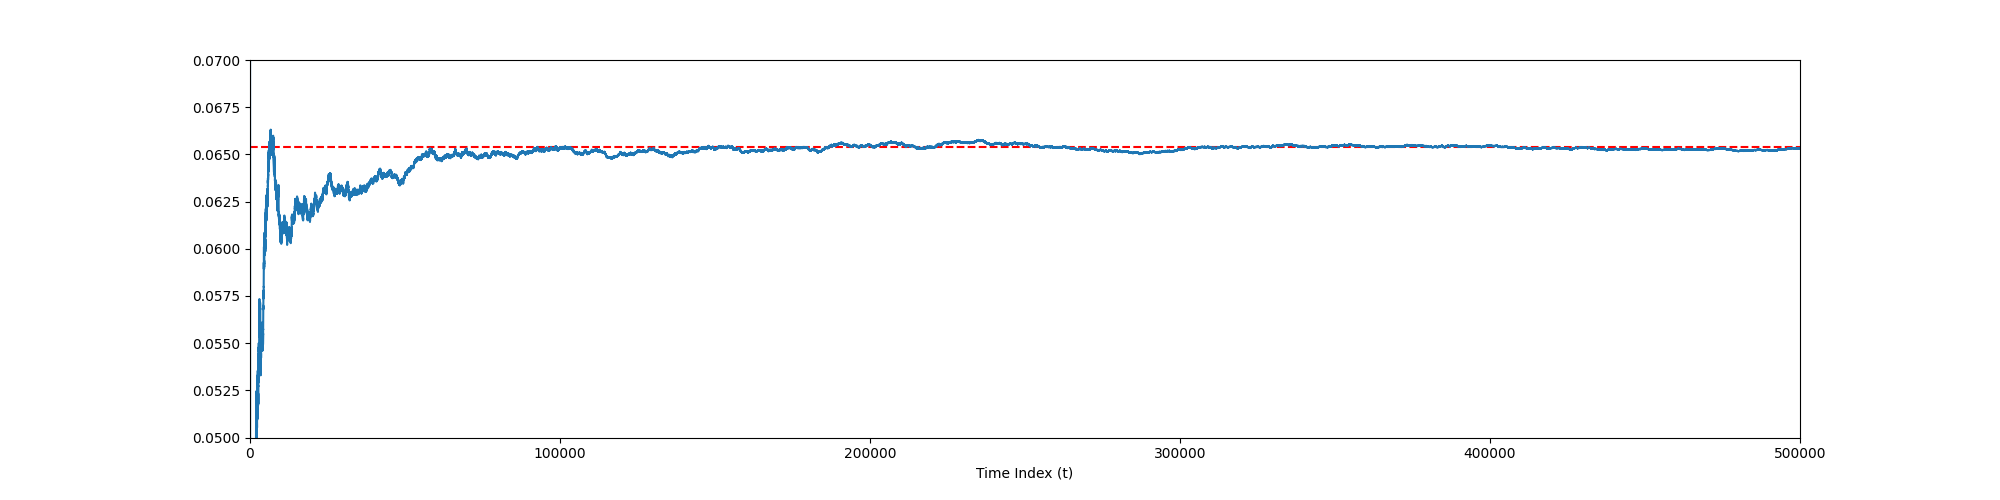
\includegraphics[scale=0.35]{images/consistency.png}
  \caption{Consistency of Bayes factor.
The blue line shows $\log(BF_{10}(\bx_{1:t}))/t$ and the red dashed line shows $D_{KL}(p(\cdot|\btheta_\star)||p(\cdot||\btheta_0)) = 0.0654$.}
    \label{fig:lbf}
  \end{figure}
  In the following simulation we demonstrate the control over false positives provided by the proposed test.
In addition, we demonstrate how continuously monitoring experiments can result in an incredibly large number of false positives when misusing a Chi-squared test.
This is easiest to visualize in an example with one treatment group with assignment probability denoted $\rho$.
The assignment is therefore a $\text{Bernoulli}(\rho)$ random variable, but sticking with the general framework developed earlier, the assignment outcome is $\text{Multinomial}(1,\btheta)$ random variable with $\btheta = [(1-\rho)\, \rho]$.
The Bayes factor in this case is then just a function of the sufficient statistic $\sum_{i=1}^t x_{i,1}$, or equivalently, $\hat{\rho}(\bx_{1:t}) = 1/t \sum_{i=1}^{t} x_{i,1}$, given by
\begin{equation}
  \label{eq:bayes_factor}
 BF_{10}(\bx_{1:t})  = \frac{\Gamma(\alpha_{0,0}+\alpha_{0,1})}{\Gamma(\alpha_{0,0}+\alpha_{0,1}+t)}\frac{\Gamma(\alpha_{0,0} + t-t\hat{\rho}(\bx_{1:t} ))\Gamma(\alpha_{0,1} + t\hat{\rho}(\bx_{1:t} )) }{\Gamma(\alpha_{0,0} )+\Gamma(\alpha_{0,1} )}\frac{1}{\theta_{0,0}^{t-t\hat{\rho}(\bx_{1:t})}\theta_{0,1}^{t\hat{\rho}(\bx_{1:t})}}.
\end{equation}
  Rejection of the null when the posterior odds $O_t(\btheta_0)$ exceeds $1/u$, is equivalent to rejecting the null whenever the test statistic $\hat{\rho}(\bx_{1:t})$ falls outside a certain interval.
This interval for $\btheta_0 = [\frac{1}{2}\, \frac{1}{2}]$, $\balpha_0 = 100\btheta_0 $, and $u=0.05$ is shown along with the interval for the Chi-squared test is shown in figure \ref{fig:critical}.
\begin{figure}[H]
  \centering
  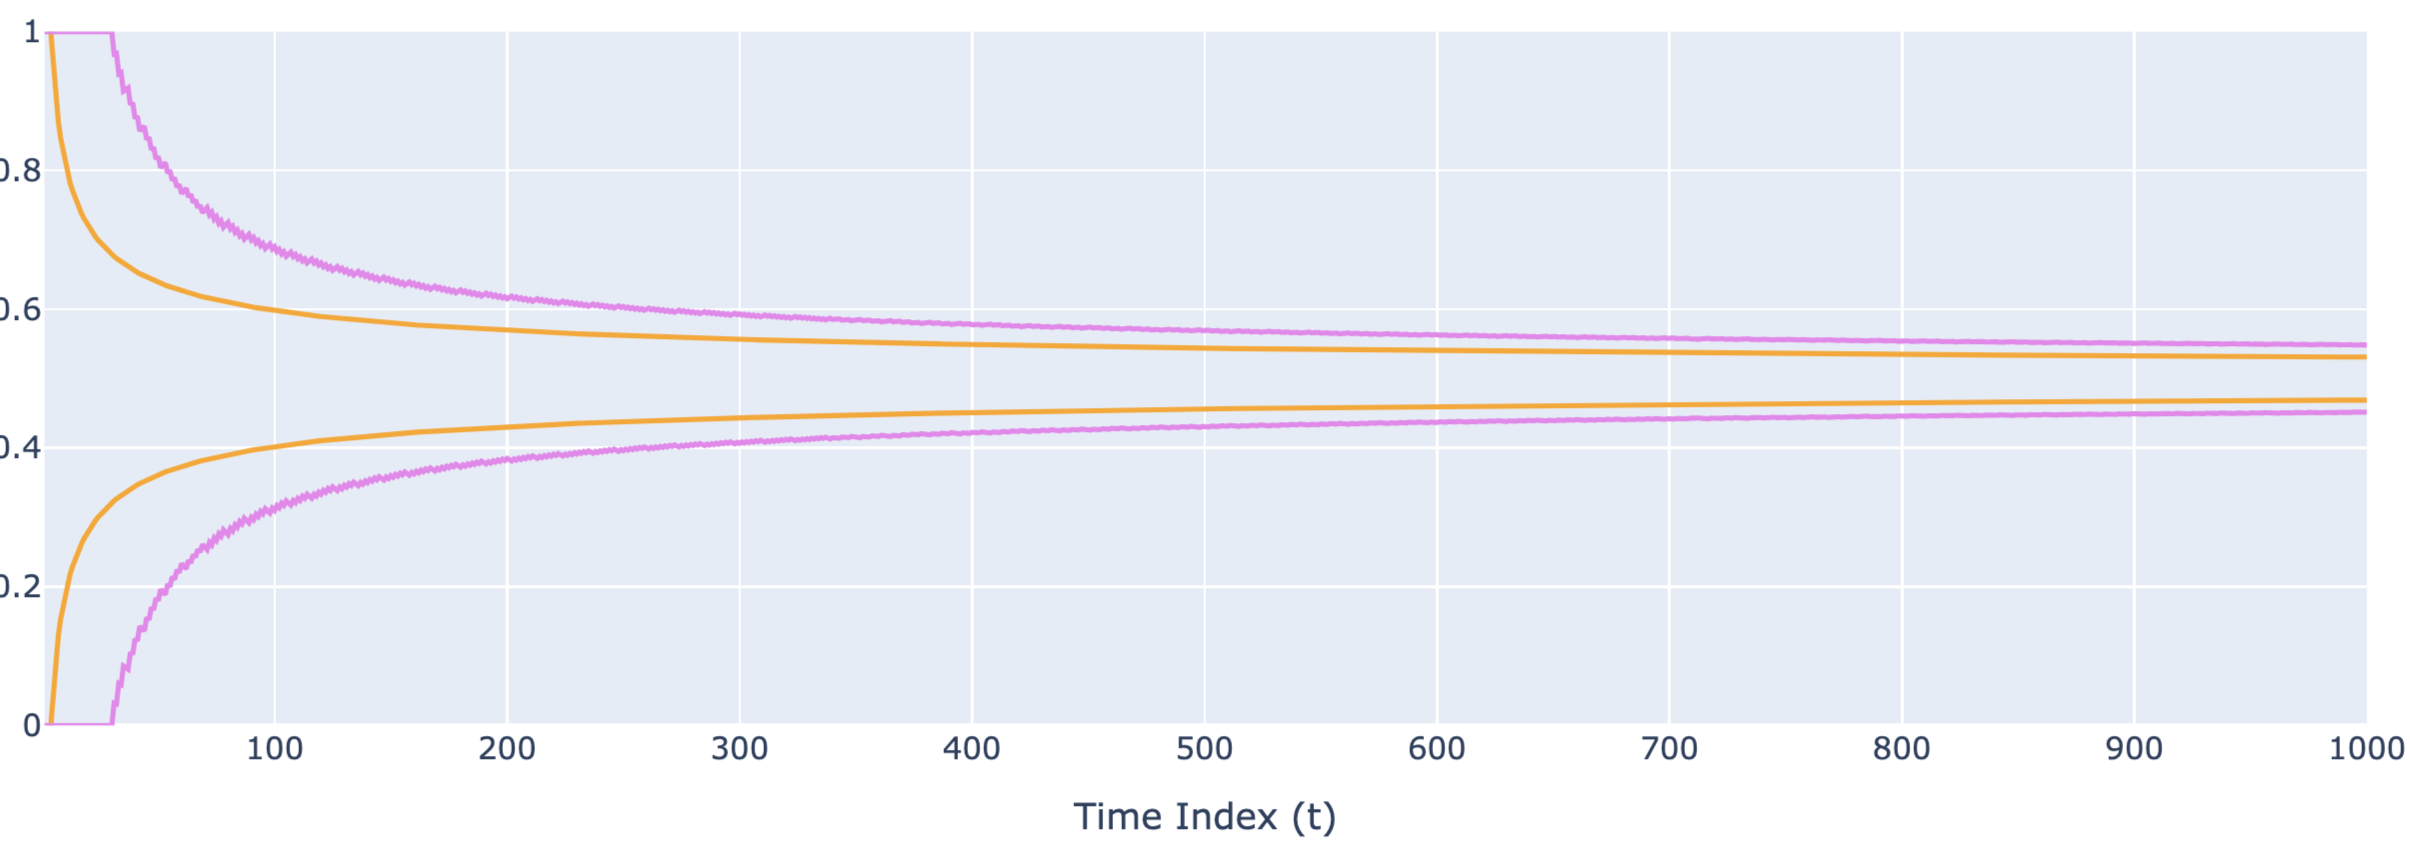
\includegraphics[scale=0.35]{images/critical_regions.png}
  \caption{Rejection boundaries for the proposed test ($\balpha_0 = 100\btheta_0$) in magenta and the Chi-squared test in orange for testing the null hypothesis $\btheta_0 = [\frac{1}{2} \, \frac{1}{2}]$ at a $u=0.05$ level.
}
    \label{fig:critical}
  \end{figure}
  An important observation is that the rejection region at any time $t$ for the proposed test is a subset of that of the Chi-squared test.
In other words, the Chi-squared test would declare a result ``significant'' at the $u=0.05$ level ``sooner'' than the proposed test.
This has to be the case, for if the proposed test were significant as often as the Chi-squared test, then the proposed test would have just as many false positives under continuous monitoring.
  
  To illustrate this point further, 100 datasets were simulated under the null hypothesis up to $t=1000$.
The Chi-squared ($u=0.05$) test was applied after every observation and by $t=1000$ 44 out of the 100 datasets resulted in the erroneous rejection of the null hypothesis.
If left to run for longer, the total number of false positives would surely increase beyond 44.
This is shown in figure \ref{fig:chi_fp}.
  \begin{figure}[h!]
  \centering
  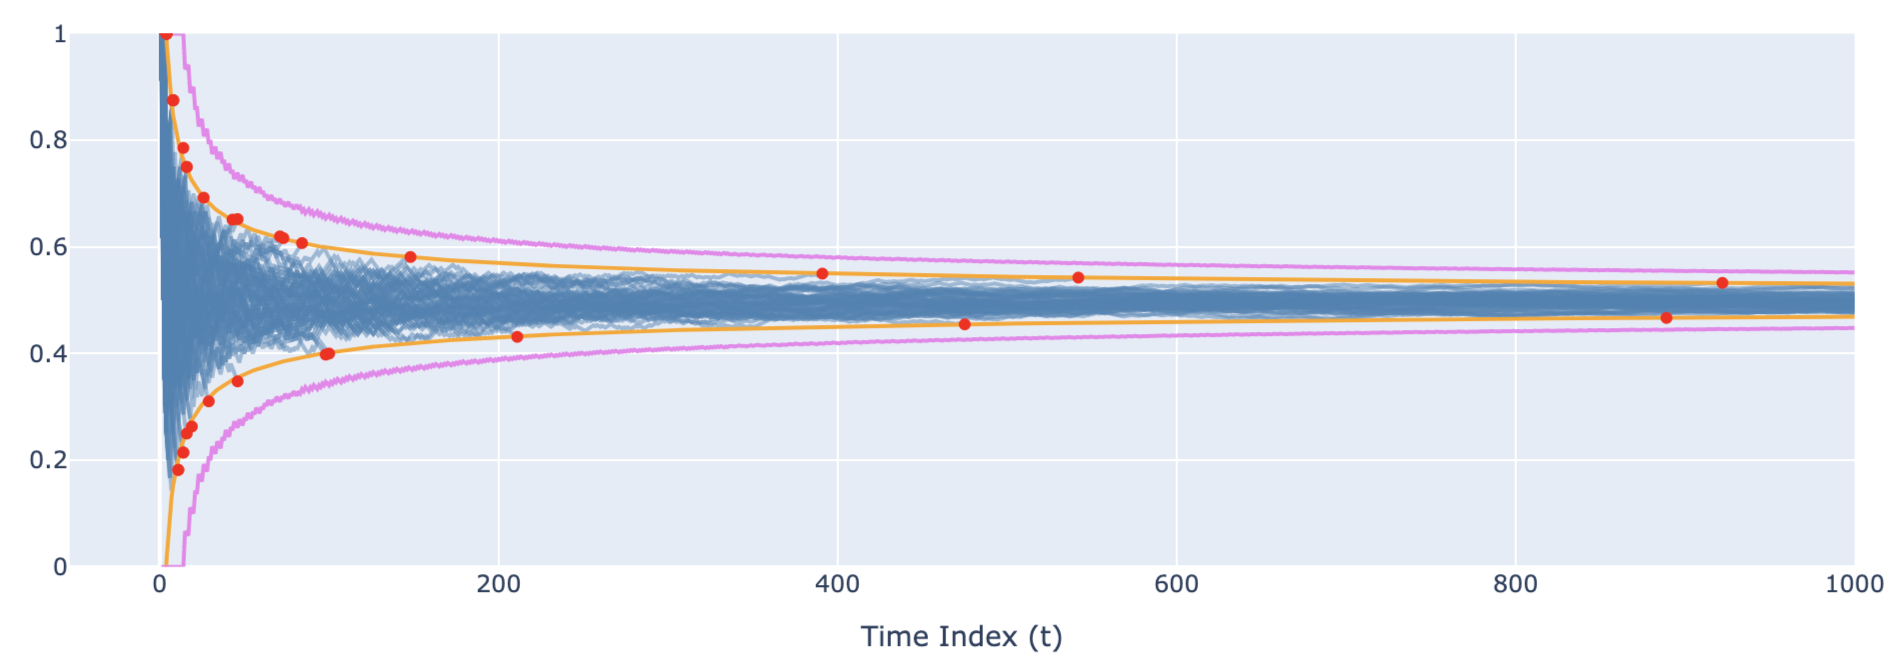
\includegraphics[scale=0.35]{images/chi_fp.png}
  \caption{Simulation Study of False Positives produced by continuously monitoring with a Chi-squared test.
The orange and magenta curves are the same as in figure \ref{fig:critical}.
Each blue trace is an independent simulation of $\hat{\rho}(\bx_{1:t})$ up until $t=1000$ or the first $t$ for which it crosses the rejection boundary of the Chi-squared test,visualized with a red dot, whichever comes sooner.
}
    \label{fig:chi_fp}
  \end{figure}
  The simulation can be repeated, using the same random number seed, to demonstrate the control over false positives of the proposed test.
Under identical conditions, the proposed test resulted in 2 out of 100 false positives, illustrated in figure \ref{fig:ssrm_fp}.
    \begin{figure}[H]
  \centering
  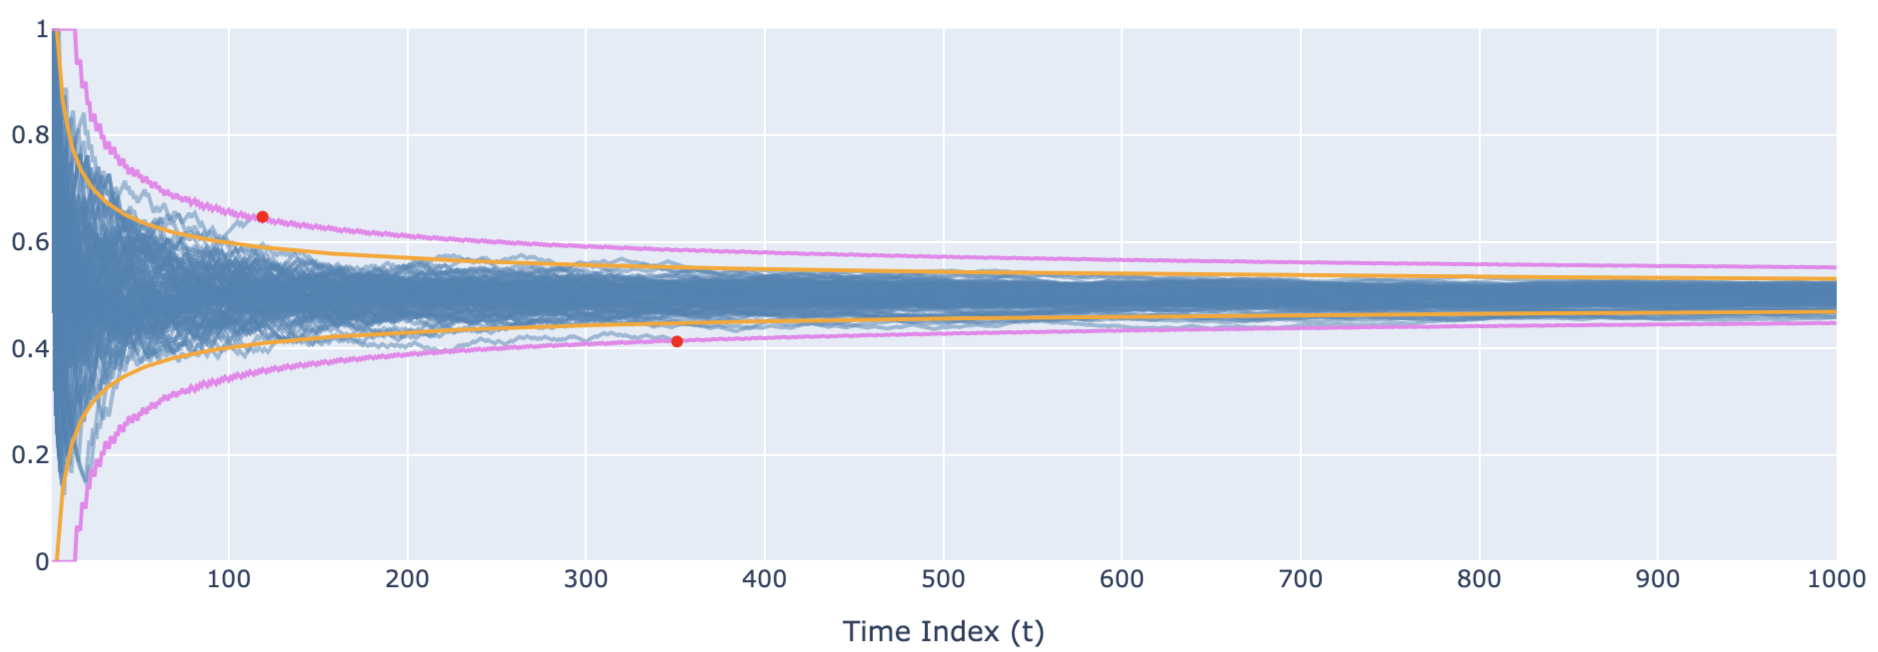
\includegraphics[scale=0.35]{images/ssrm_fp.png}
  \caption{Simulation Study of False Positives produced by continuously monitoring with the proposed test.
The orange and magenta curves are the same as in figure \ref{fig:critical}.
Each blue trace is an independent simulation of $\hat{\rho}(\bx_{1:t})$ up until $t=1000$ or the first $t$ for which it crosses the rejection boundary of the Chi-squared test,visualized with a red dot, whichever comes sooner.
}
    \label{fig:ssrm_fp}
  \end{figure}
  We now turn our attention to visualizing the main value add of the proposed test, namely, to reject the null hypothesis quickly.
Suppose an experiment has been designed and a sample size calculation has determined that $1000$ datapoints must be collected.
The intended treatment assignment probability is 0.5, yet due to a bug in the code introducing bias in the assignment mechanism, or a missing data mechanism for the control group, the probability of recording an observation from the treatment is in fact 0.6.
  Figure \ref{fig:ssrm_reject} demonstrates that the proposed test rapidly rejects the null way before the end of the experiment, saving further units from entering an incorrectly executed experiment.
      \begin{figure}[H]
  \centering
  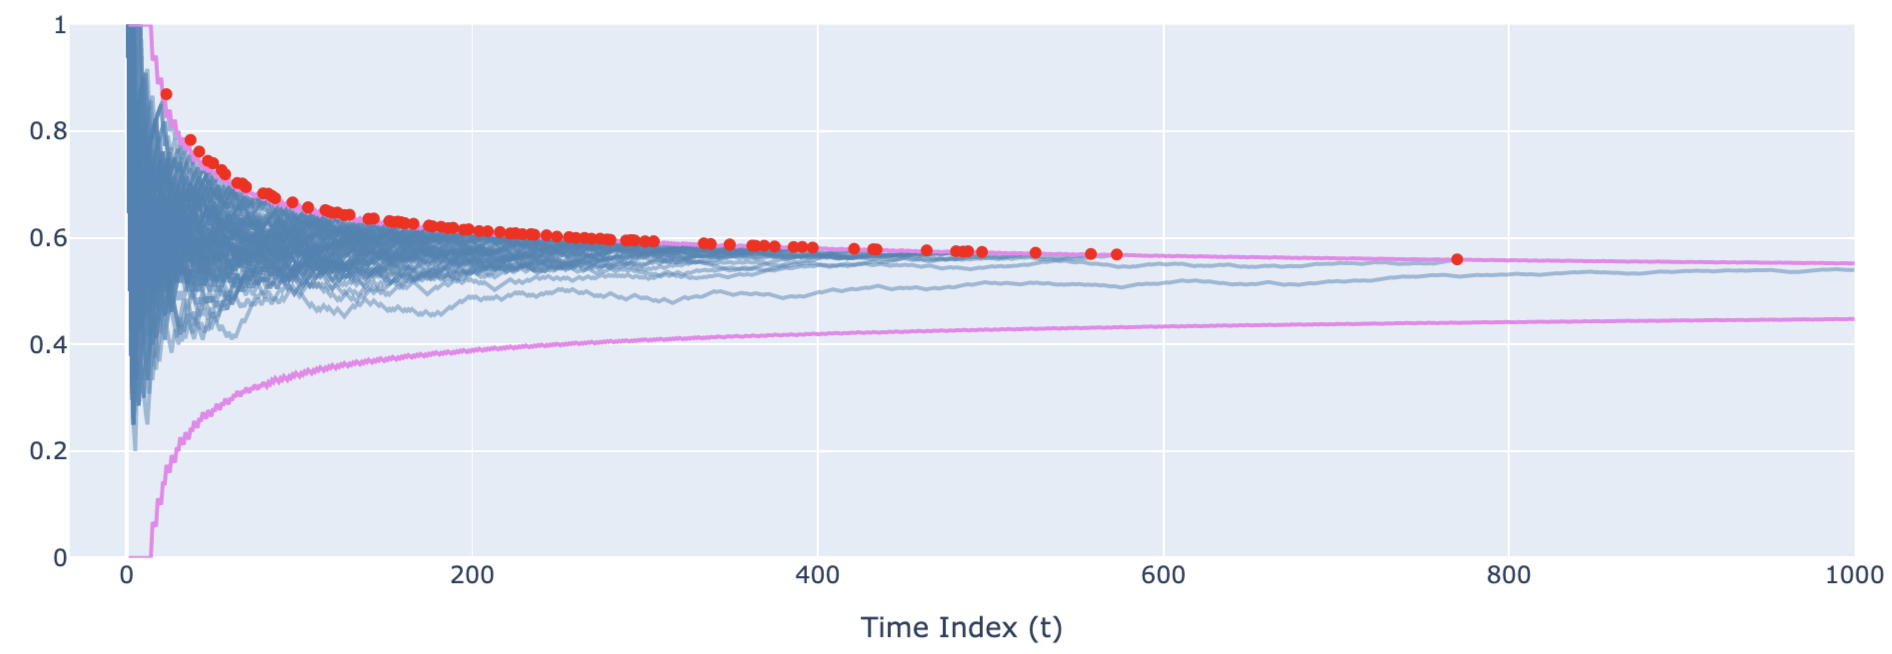
\includegraphics[scale=0.35]{images/ssrm_reject.png}
  \caption{Simulation Study of time to reject the null under the proposed test.
The magenta curve is the same as in figure \ref{fig:critical}.
Each blue trace is an independent simulation of $\hat{\rho}(\bx_{1:t})$ up until $t=1000$ or the first $t$ for which it crosses the rejection boundary of the Chi-squared test,visualized with a red dot, whichever comes sooner.
}
    \label{fig:ssrm_reject}
  \end{figure}
  \noindent To add some intuition to figure \ref{fig:ssrm_reject}, it can be shown that the rection region at time $t$ converges to $[0,1]\setminus \btheta_0$, yet $\btheta_0 \rightarrow \btheta_\star$ $a.s.$ as $t\rightarrow \infty$.
In this specific example, the region of indifference degenerates onto $\lbrace 0.5 \rbrace$, yet $\hat{\rho}(\bx_{1:t})$ converges to 0.6 almost surely as $t \rightarrow \infty$ by the strong law of large numbers, which provides an alternative argument to Theorem~\ref{thm:consistency} for rejecting the null almost surely.
  \section{Discussion}
  \label{sec:discussion}
The main purpose of this paper was to provide a tool that can be used sequentially to detect practical implementation errors in an experiment, such as identifying biased assignment mechanisms or surfacing missing data mechanisms which are frequently observed in online controlled experiments.
The proposed test permits optional stopping and continuation, allowing experiments to be continuously monitored.
The hypothesis can be tested, therefore, after every single data point so as to detect errors as quickly as possible.
While Bayesian in construction, we provided sequential guarantees of the frequentist Type-I error probability and also studied the power of this test through a combination of theoretical results and simulation studies.
While our application of detecting errors in simply randomized experiments focussed on a specific Multinomial-Dirichlet test, the same mathematical techniques can be obviously used to generalize these results to other Bayesian tests.
With generalization in mind, there are some remaining comments and ideas for future work.

We first address the differences in the purely Bayesian approach and the test proposed here.
For instance, under the same stopping rule of rejecting the null when the posterior odds exceed $1/u$, a Bayesian would report a (Bayesian) Type-I error probability of $u/(1+u)$, whereas a frequentist would report a slightly larger (frequentist) Type-1 error probability of $u$.
One important distinction is that the latter does not depend at all on the realized data, whereas the former depends on the data actually observed.
In this sense, the Bayesian answer is a data dependent error probability.
The intuition that one is less likely to believe an outcome is a false positive as the test statistic becomes more extreme leads to the notion of conditional frequentist testing (\cite{kiefer}).
In conditional frequentist testing one reports the data dependent Type-I error probability $\alpha(s) = \mathbb{P}(\text{Type I error} | S(X) = s)$ for a suitable conditioning statistic $S(X)$.
The challenge in conditional frequentist testing is to find an appropriate conditioning statistic $S(X)$.
\cite{conditional_frequentist_composite} showed that the Bayesian Type I error probabilities are equal to the conditional frequentist Type I error probabilities by choosing the conditioning statistic to be a function of the Bayes factor.

We note that the confidence sequences described in Theorem~\ref{thm:confidence_sequence} share a connection with other Bayesian intervals discussed in the literature.
To see this it is necessary to express the Bayes factor in terms of the Savage-Dickey density ratio (\cite{dickey}) as
\begin{equation}
    B(\bx_{1:t}|\btheta_0) = \frac{p(\btheta_0| M_1)}{p(\btheta_0|\bx_{1:t},M_1)}.
\end{equation}
This, with $O_0(\btheta_0)=1$, implies that $I_t(u) = \lbrace \btheta \in \triangle^d : O_t(\btheta) \leq 1/u \rbrace = \lbrace \btheta  \in \triangle^d : p(\btheta| M_1)\leq p(\btheta|\bx_{1:t}, M_1)/u \rbrace $, which is identified as the Bayesian \textit{support interval} proposed by \cite{support_interval}.
The authors proposed this as an alternative to the more commonly reported Bayesian credible intervals, argueing that the support interval is based on evidence in the data (how the data changes belief), whereas credible intervals are based on posterior belief directly.
These intervals have some intuitive appeal as they are the parameter values for which their posterior density has increased beyond some factor of their prior density after observing the data.
We are the first, however, to identify the sequential frequentist coverage probabilities, in the sense of Theorem~\ref{thm:confidence_sequence}, of these support intervals.


\bibliographystyle{plainnat}
\bibliography{sample}


\appendix
\section{Posterior Odds Updating Rules}
\label{app:posterior_odds}
The Bayes factor after $t$ observations is analytically tractable, given by
\begin{equation}
  \label{eq:bayes_factor}
 \frac{p(\bx_{1:t}|M_1)}{p(\bx_{1:t}|M_0)} = \frac{\Gamma(\sum_{j=1}^{d} \alpha_{0,j})}{\Gamma(\sum_{j=1}^{d} \alpha_{0,j} + \sum_{i=1}^{t}x_{i,j})}\frac{\prod_{j=1}^{d}\Gamma(\alpha_{0,j} + \sum_{i=1}^{t}x_{i,j} )}{\prod_{j=1}^{d}\Gamma(\alpha_{0,j} )}\frac{1}{\prod_{j=1}^{d} \theta_{0,j}^{\sum_{i=1}^{t}x_{i,j}}}.
\end{equation}
It is helpful to introduce some further notation to explicitly express the sequential nature inherent to the problem.

The Posterior odds in favour of $M_1$ to $M_0$ after observing $\bx_{1:t}$ is defined as
\begin{align}
  \label{eq:general_posterior_odds}
  \frac{p(M_1|\bx_{1:t})}{p(M_0|\bx_{1:t})}  &= \frac{\int p(\bx_{1:t}|\btheta,M_1)p(\btheta,M_1)d\btheta}{p(\bx_{1:t}|M_0)}\frac{P(M_1)}{P(M_0)},\\
                      &=\frac{p(\bx_{1:t}|M_1)}{p(\bx_{1:t}|M_0)}\frac{p(M_1)}{p(M_0)},\\
                      &=\frac{\prod_{i=1}^{t}p(\bx_i|\bx_{1:i-1}|M_1)}{\prod_{i=1}^{t}p(\bx_i|\bx_{1:i-1}|M_0)}\frac{p(M_1)}{p(M_0)},\\
                      &=\frac{p(\bx_t|\bx_{1:t-1},M_1)}{p(\bx_t|\bx_{1:t-1},M_0)} \frac{p(M_1|\bx_{1:t-1})}{p(M_0|\bx_{1:t-1})},\\
    &=\frac{\int p(\bx_t|\btheta,\bx_{1:t-1},M_1)p(\btheta|\bx_{1:t-1},M_1)d\btheta}{p(\bx_t|\bx_{1:t-1},M_0)}  \frac{p(M_1|\bx_{1:t-1})}{p(M_0|\bx_{1:t-1})} ,
\end{align}
where the last expression stresses the recursive definition of the Posterior odds factor in terms of products of posterior predictive densities.
The posterior distribution of $\btheta| \bx_{1:t}, M_1 \sim \text{Dirichlet}(\balpha_t)$ where $\balpha_t = \balpha_{t-1}+\bx_t$ with $\balpha_0$ the initial prior parameter choice.
The posterior predictive densities are easily computed as
\begin{equation}
  \label{eq:posterior_predictive_m1}
   p(\bx_t|\bx_{1:t-1},M_1) = \frac{ \Gamma(\sum_i x_{t,i}+ 1)}{\prod_i \Gamma(x_{t,i} + 1)} \frac{\Gamma(\sum_i \alpha_{t-1,i})}{\prod_i \Gamma(\alpha_{t-1,i})} \frac{\prod_i \Gamma(\alpha_{t-1,i} + x_{t,i})}{\Gamma(\sum_i \alpha_{t-1,i} + x_{t,i})},
\end{equation}
and
\begin{equation}
  \label{eq:posterior_predictive_m2}
   p(\bx_t|\bx_{1:t-1},M_0) = \frac{ \Gamma(\sum_i x_{t,i} + 1)}{\prod_i \Gamma(x_{t,i} + 1)} \prod \theta_{0,i}^{x_{t,i}}.
 \end{equation}
 It will be useful later on to introduce the following notation for the posterior odds at time $t$ as $O_t(\btheta_0)$, which explicitly states the value of $\theta$ under the null hypothesis.
The recursive definition of the posterior odds can then be expressed as
\begin{align}
  O_{t}(\btheta_0) &= \frac{\Gamma(\sum_i \alpha_{t-1,i})}{\Gamma(\sum_i \alpha_{t-1,i} +  x_{t,i})} \frac{\prod_i \Gamma(\alpha_{t-1,i} + x_{t,i})}{\prod_i \Gamma(\alpha_{t-1,i})} \frac{1}{\prod_i \theta_{0,i}^{x_{t,i}}}  O_{t-1}(\btheta_0),\\
\end{align}
with
\begin{align}
  \label{eq:alpha_update}
  \balpha_{t}&= \balpha_{t-1}+\bx_t.
\end{align}
and initial value
\begin{align}
  \label{eq:bayes_factor_seed}
O_0(\btheta_0) = \frac{p(M_1)}{p(M_0)}.
\end{align}


\section{Uniform Bounds on the Type-I Error}
\label{app:type_1_error}
To result follows from the application of the following two lemmas.
\begin{lemma}(Martingale property of posterior odds under the null hypothesis)
  
  \noindent Let $\bx_i,$ be a sequence of $\text{Multinomial}(n_i,\btheta)$ random variables and consider the sequence of posterior odds $O_t(\btheta_0)$ defined as in equation \eqref{eq:update_rule} with $O_0(\btheta_0)=1$, then $O_t(\btheta_0)$ is a nonnegative martingale under $M_0$.
  \label{lem:posterior_odds_martingale}
    \end{lemma}
  \begin{proof}
  \begin{align*}
    E_{M_0}[O_{t+1}(\btheta_0)|\mathcal{F}_t]  &= \int \frac{p(\bx_{t+1}|\bx_{1:t},M_1)}{p(\bx_{t+1}|\bx_{1:t},M_0)} O_{t}(\btheta_0) p(\bx_{t+1}|\bx_{1:t},M_0) d\bx_{t+1}\\
    &=  O_{t}(\btheta_0) \int p(\bx_{t+1}|\bx_{1:t},M_1) d\bx_{t+1}\\
    &=  O_{t}(\btheta_0),
  \end{align*}
  where $\mathcal{F}_{t} = \sigma(x_1,x_2,\dots, \bx_t)$
\end{proof}

\begin{lemma}(Ville's Maximal Inequality)
  
\label{lem:durrett}
  \noindent If $Z_{t}$ is a nonnegative supermartingale with respect to the filtration $\mathcal{F}_t$, then
  \begin{equation}
    \label{eq:durrett}
    \mathbb{P}[\exists t \in \mathbb{N}\cup \lbrace 0 \rbrace : Z_t \geq u] \leq \frac{Z_0}{u}
  \end{equation}
\end{lemma}
\begin{proof}
  See Proof 6.1 of \cite{howard}
\end{proof}
The result of the Theorem is obtained by using lemma \ref{lem:posterior_odds_martingale} to establish that the posterior odds $O_t(\btheta_0)$ are a nonnnegative supermartingale under the null hypothesis, and using this obseravtion in lemma \ref{lem:durrett} together with  $O_0(\btheta_0) = 1$  to obtain the main inequality of the Theorem.
\section{Asymptotic Properties of Bayes Factors}
\label{app:asymptotics}
We first narrow the focus of a general result found in Theorem~1 of \cite{walker}.
Let $D_{KL}(p(\cdot|\btheta_\star)||p(\cdot|\btheta) )$ denote the Kullback-Leibler divergence of a multinomial distribution indexed by a parameter $\theta$ from the true multinomial distribution with true parameter $\btheta_{\star}$.
Moreover let $D_{KL}(p(\cdot|\btheta_\star)||p(\cdot|\bx_{1:t}, M_j) )$ denote the KL divergence of the posterior predictive distribution under model $j$ at time $t$ from the true multinomial distribution.
Let $A(q) = \lbrace \btheta \in \triangle^d : D_{KL}(p(\cdot|\btheta_\star)||p(\cdot|\btheta) ) < q \rbrace$
\begin{lemma}
  \label{lemma:walker}
  If $\int_{A(q)} p(\btheta|M_j) d\btheta > 0$ only for, and for all, $q > \delta_j$, and $\lim \inf_t D_{KL}(p(\cdot|\btheta_\star)||p(\cdot|\bx_{1:t}, M_j) ) \geq \delta_j$ a.s.
then
  \begin{equation}
    \label{eq:bayes_factor_convergence}
    \frac{1}{t} \log B_{10}(\bx_{1:t}) \rightarrow \delta_0 - \delta_1,
  \end{equation}
  provided that $\sum_t \frac{1}{t^2} \left( \mathbb{V}[\log \frac{p(\bx_t|\bx_{1:t-1},M_j)}{p(\bx_t|M_\star )}]\right) < \infty$.
\end{lemma}
\begin{proof}
  For $j=0,1$ consider the following martingale
  \begin{align*}
    \label{eq:walker_martingale}
    S_{jt} =& \sum_{i=1}^{t} \log \frac{p(\bx_i|\bx_{1:i-1},M_j)}{p(\bx_i|M_\star)} + D_{KL}(p(\cdot|\btheta_\star)||p(\cdot|\bx_{1:i-1}, M_j) ),\\
    =& -\log \frac{p(\bx_t|M_\star)}{p(\bx_t|\bx_{1:t-1},M_j)} + D_{KL}(p(\cdot|\btheta_\star)||p(\cdot|\bx_{1:t-1}, M_j) ) +\\
    &S_{jt-1},\\
  \end{align*}
  from which it follows that $\mathbb{E}[S_{jt}|\mathcal{F}_t] = S_{jt-1}$ with $\mathcal{F}_t = \sigma(x_1,\dots,x_{t-1})$.
From the assumption that  $\sum_t \frac{1}{t^2} \left( \mathbb{V}[\log \frac{p(\bx_t|\bx_{1:t-1},M_j)}{p(\bx_t|M_\star )}]\right) < \infty$, it follows that $S_{jt}/t \rightarrow 0$ a.s.
and consequentially
  \begin{align*}
    \frac{1}{t} \log \frac{p(\bx_{1:t}|M_j)}{p(\bx_{1:t}|M_\star)} + \frac{1}{t}\sum_{i=1}^t  D_{KL}(p(\cdot|\btheta_\star)||p(\cdot|\bx_{1:t-1}, M_j) )\rightarrow 0.
  \end{align*}
  From the additional assumption of $\lim \inf_t D_{KL}(p(\cdot|\btheta_\star)||p(\cdot|\bx_{1:t}, M_j) ) \geq \delta_j$ a.s.
, it follows that
  \begin{align*}
    \lim \sup   \frac{1}{t} \log \frac{p(\bx_{1:t}|M_j)}{p(\bx_{1:t}|M_\star)} \leq - \delta_j \hspace{1cm} a.s.
  \end{align*}
  With the Kullback Leibler property of the prior it follows that
  \begin{align*}
     \lim \inf   \frac{1}{t} \log \frac{p(\bx_{1:t}|M_j)}{p(\bx_{1:t}|M_\star)} \geq - \delta_j \hspace{1cm} a.s.
  \end{align*}
  from \cite{barron}.
It follows that
    \begin{align*}
     \lim   \frac{1}{t} \log \frac{p(\bx_{1:t}|M_j)}{p(\bx_{1:t}|M_\star)} \rightarrow - \delta_j \hspace{1cm} a.s.
    \end{align*}
    Combining this result for models $M_1$ and $M_0$ completes the proof.
\end{proof}

The application of this lemma to the multinomial Dirichlet model is then straight forward.
Note that under model $M_0$, the prior on $\theta$ is a point mass at $\btheta_0$.
Let the KL divergence of the null model from the true model be denoted $\delta_0$, it is clear that $\int_{A(q)} p(\btheta|M_0) d\btheta = 0$ if $q<\delta_0$ and 1 otherwise.
Hence KL divergence of the null $\btheta_0$ from the true $\btheta_\star$ is the relevant $\delta_0$ for model $M_0$ in lemma \ref{lemma:walker}.
The value of $\delta_1$ for the Dirichlet prior under model $M_1$, however, is zero.


\section{Manipulating the Rejection Region}
Our goal is to find some event $\mathcal R_n'\subseteq \mathcal R_n$ that is more amenable to computation; this allows us to obtain a bound on the power since
$\mathbb{P}(\mathcal R_n) \geq \mathbb{P}(\mathcal R_n')$.
The proof is by explicit construction, and we begin by deriving a lower bound on 
$
 \frac{\Beta(\balpha + \bS_n)} {\Beta(\balpha)} \btheta_0 ^{-\bS_n}
$.
\begin{lemma}\label{lem:beta.lower.bound}
  For all $\balpha$ in the positive orthant,
  \begin{equation*}
    (2\pi)^{\frac{d-1}{2}}
    \frac{\prod_{i=1}^d \alpha_i^{\alpha_i - 1/2}}{|\balpha|^{|\balpha|-1/2}e^{\frac{1}{12|\balpha|}}} \leq  \Beta(\balpha) \leq 
(2\pi)^{\frac{d-1}{2}}
    \frac{\prod_{i=1}^d \alpha_i^{\alpha_i - 1/2}e^{\frac{1}{12\alpha_i}}}{|\balpha|^{|\balpha|-1/2}} 
  \end{equation*}
\end{lemma}
\begin{proof}
  We first recall a Stirling-type set of lower and upper bounds on the gamma function
\begin{equation}
(2\pi)^{\frac{1}{2}}x^{x-\frac{1}{2}}e^{-x}
  \leq \Gamma(x) \leq (2\pi)^{\frac{1}{2}}x^{x-\frac{1}{2}}e^{-x}e^{\frac{1}{12x}},
\end{equation}
which can be verified in \cite{specialfunctions}.
Together these bounds provide a bound on the error of the lower bound.
In particular $|\log \Gamma(x) - \frac{1}{2}\log (2\pi) - (x-\frac{1}{2})\log x + x| \leq \frac{1}{12x}$, which shows
that the lower bound error will become vanishingly small as $x\rightarrow \infty$, which is the case for our application. 
These ideas follow through to lower bounding the Beta function. The lower bound on the Beta function follows by applying the lower bound to the Gamma funcitons
in the numerator and the upper bound to the Gamma function in the denominator. The upper bound follows similarly.
\end{proof}
\noindent We can now finish the proof of Theorem~\ref{thm:calRprime}.
\begin{proof}
If a lower bound on the odds is greater than $1/u$, then the odds itself is greater than $1/u$. Let's first
establish a lower bound on the odds using lemma \ref{lem:beta.lower.bound}.
\begin{align*}
    \frac{\Beta(\balpha + \bS_n)}
  {\Beta(\balpha)} \theta_0^{-\bS_n}
  &\geq
  (2\pi)^{\frac{d-1}{2}}
    \frac{ \prod_i (\alpha_i+S_i^n)^{\alpha_i + S_i^n-1/2}}
    {(|\balpha|+n)^{|\balpha| + n - 1/2}}
    \frac{ \theta_0^{-\bS_n}}{e^{\frac{1}{12(|\balpha|+n)}}\Beta(\balpha)}\\
  &=
  (2\pi)^{\frac{d-1}{2}}
    \frac{ \prod_i (\alpha_i+S_i^n)^{\alpha_i + S_i^n-1/2}}
    {(|\balpha|+n)^{|\balpha| + n - 1/2}}
    \prod_i \left( \frac{\hat{\theta}^n_i}{\theta_{0,i}} \right)^{S^n_i}
    \frac{1}{\prod_i (\hat{\theta}^n_i)^{S^{n}_{i}}}
    \frac{ 1}{e^{\frac{1}{12(|\balpha|+n)}}\Beta(\balpha)}\\
  &=
  (2\pi)^{\frac{d-1}{2}}
    \frac{ \prod_i (\alpha_i+S_i^n)^{\alpha_i + S_i^n-1/2}}
    {(|\balpha|+n)^{|\balpha| + n - 1/2}}
    e^{n \KL(\hat\btheta_n|| \btheta)}
    \frac{n^{n}}{\prod_i (S^n_i)^{S^{n}_{i}}}
    \frac{ 1}{e^{\frac{1}{12(|\balpha|+n)}}\Beta(\balpha)}\\
  &=
  (2\pi)^{\frac{d-1}{2}}
    \frac{ \prod_i (\alpha_i+S_i^n)^{\alpha_i + S_i^n-1/2}}
    {\prod_i (S^n_i)^{S^{n}_{i}}}
    e^{n \KL(\hat\btheta_n|| \btheta)}
    \frac{n^{n}}{(|\balpha|+n)^{|\balpha| + n - 1/2}}
    \frac{ 1}{e^{\frac{1}{12(|\balpha|+n)}}\Beta(\balpha)}\\
  &>
  (2\pi)^{\frac{d-1}{2}}
    e^{n \KL(\hat\btheta_n|| \btheta)}
    \frac{n^{n}}{(|\balpha|+n)^{|\balpha| + n - 1/2}}
    \frac{ 1}{e^{\frac{1}{12(|\balpha|+n)}}\Beta(\balpha)}\\
\end{align*}
The first inequality follows from the lower bound derived in lemma \ref{lem:beta.lower.bound}.
The second inequality follows from
\begin{align*}
  \frac{ \prod_i (\alpha_i+S_i^n)^{\alpha_i + S_i^n-1/2}}
  {\prod_i (S^n_i)^{S^{n}_{i}}} \geq 1,
\end{align*}
so long as $\alpha_i \geq 1/2$ for each $i$. We also note that this term converges to unity as $n\rightarrow \infty$, and
so the bound is expected to be increasingly good for large $n$.
Now consider the simpler rejection region
\begin{align*}
  \mathcal{R}_n' &= \left\{ \bx_{1:n} : 
  \KL(\hat\btheta_n|| \btheta) > \frac{1}{n}\left( \log \frac{\Beta(\balpha)}{u} +(|\balpha|+n-1/2)\log(|\balpha|+n)-n\log n + \frac{1}{12(|\balpha|+n)} - \frac{d-1}{2}\log 2\pi\right)\right\}\\
  &= \left\{ \bx_{1:n} : 
  (2\pi)^{\frac{d-1}{2}}
    e^{n \KL(\hat\btheta_n|| \btheta)}
    \frac{n^{n}}{(|\balpha|+n)^{|\balpha| + n - 1/2}}
    \frac{ 1}{e^{\frac{1}{12(|\balpha|+n)}}\Beta(\balpha)} > \frac{1}{u} \right\}\\
   &\subset \left\{ \bx_{1:n} : 
    \frac{\Beta(\balpha + \bS_n)}
  {\Beta(\balpha)} \theta_0^{-\bS_n} > \frac{1}{u}
\right\}\\
    &= \mathcal{R}_n\\
\end{align*}
It is reassuring to observe that $|\balpha|$ always appears in combination with $n$. Recall if we choose $\alpha=k\theta_0$, then $|\balpha|=k$ is interpreted as the prior sample size in a Multinomial-Dirichlet model.
The sum $|\balpha|+n$ can be interpreted as the total samples, from the data and the prior.

Let us write $\mathcal{R}_n' = \left\{ \bx_{1:n} : \KL(\hat\btheta_n|| \btheta) > \underline{D}_n(u,\balpha) \right\}$, then $\underline{D}_n(u,\balpha) \sim \mathcal{O}((1/n)\log n)$.
To see this note that 
\begin{align*}
  (|\balpha|+n-1/2)\log(|\balpha|+n)-n\log n < (|\balpha|-1/2)\log(|\balpha|+n) + |\alpha|/n,
\end{align*}
where we have used the mean value theorem to write $\log(|\balpha|+n) = \log(n) +  |\balpha|/c$ for some $c\in (n, n+|\balpha|)$, 
which can be upper bounded by $\log(n) + |\balpha|/n$, which can be interpreted as the logarithmic function being bounded from above by the tangent at $n$.
\end{proof}

\section{Lower Bounding the Stopping Time CDF}
In order to assess how quickly the proposed test is able to reject the null, we would like to obtain, or at least lower bound, the probability
or rejecting the null hypothesis by a time $n$. Denote the random stopping time of rejecting the null hypothesis as $\tau = \inf \{n : O_n(\btheta_0) > 1/u\} =\inf \{n : x_{1:n} \in \mathcal{R}'_n\}$. 
A simple lower bound can be obtained as follows
\begin{align*}
  \mathbb{P}_\btheta[\tau \leq n] &\geq \mathbb{P}_\btheta[\exists i \leq n : \bx_{1:i} \in \mathcal{R}_i]\\ 
&\geq \mathbb{P}_\btheta[\bx_{1:n} \in \mathcal{R}_n]\\ 
&\geq \mathbb{P}_\btheta[\bx_{1:n} \in \mathcal{R}'_n].\\ 
\end{align*}
The second inequality is simply stating that the probability of rejecting the null hypothesis is higher if
we apply the test after every data point up to and including time $n$, than simply applying the test at time $n$.
This makes sense, as there are simply more opportunities for the null to be rejected. 
The last inequality follows from lemma \ref{thm:calRprime}.
Note that the rejection region $\mathcal{R}_n'$ depends on $\bx_{1:n}$ only through the MLE $\hat{\btheta}(\bx_{1:n})$.
In what follows it is helpful to consider $\hat{\btheta}(x_{1:n})$ as a test statistic at time $n$,
and define a corresponding rejection region as a subset of $\triangle^d$ at time $n$.
Let this rejection region in $\triangle^d$ be denoted $T_n = \{\btheta \in \triangle^d : \KL(\btheta||\btheta_0) > \underline{D}_n(u,\balpha)\}$, then $\hat{\btheta}(x_{1:n})\in T_n$ implies
$\bx_{1:n} \in \mathcal{R}'_n$.
We now combine this with the concentration inequality of \cite{weissman2003inequalities} for the MLE of a multinomial model
\begin{align*}
  \mathbb{P}_\btheta[\hat{\btheta}_n \in C_n^\delta] \geq 1 - \delta,
\end{align*}
where $C_n^\delta = \{ \btheta \in \triangle^d : \|\btheta-\btheta_\star\|_1 \leq \sqrt{\frac{4\log \frac{2}{\delta}}{n}}\}$.
At any time we now have two sets in $\triangle^d$. 
The first is a rejection set which converges to  $\triangle^d \setminus \btheta_0$ as $n \rightarrow \infty$,
the second a set which concentrates around the true parameter $\btheta_\star$ as $n \rightarrow \infty$.
If the MLE is in the latter with high probability, and this set is totally contained inside the rejection set, then the test statistic is in the rejection set with high probability. 
This is only possible for large enough $n$ so that $\btheta_\star \in T_n$, after which one chooses the smallest $\delta$ satisfying $C_n^\delta \subset T_n$, yielding $1-\delta$ lower bound on the probability of rejection.


Because the rejection set $T_n$ is defined in terms of the KL divergence, while the concentration set $C_n^\delta$ is defined in terms of the L1-norm, we define
$T_n' = \{\btheta \in \triangle^d : \|\btheta-\btheta_0\|_1 > (1/2)\underline{D}_n(u,\balpha)\}$.
It follows from Pinsker's inequality $2\|\bx-\btheta\|_1\leq \KL(\bx||\btheta)$ that $T_n' \subset T_n$.
Let $N = \min \{n \in \mathbb{N} : \btheta_\star \in T_n'\}$, this ensures that the the true parameter is in the rejection region $T_n'$ for all subsequent $n$, around which a $C_n^\delta$ can be placed for suitably small $\delta$.
Let
\begin{equation*}
  \delta = 2e^{-\frac{n}{4}\left(\|\btheta_\star - \btheta_0\|_1-\frac{1}{2}\underline{D}_n(u,\balpha)\right)^2}
\end{equation*}
It follows for $\btheta \in C_n^\delta$, 
\begin{align*}
  \|\btheta-\btheta_0\|_1 &\geq  \|\btheta_\star - \btheta_0\|_1 - \|\btheta - \btheta_\star \|_1 \hspace{1cm}\text{(Reverse Triangle Inequality)},\\
  &\geq \sqrt{\frac{4\log \frac{2}{\delta}}{n}} - \|\btheta - \btheta_\star \|_1 \hspace{1cm} (\btheta \in C_n^\delta),\\
  &\geq \frac{1}{2}\underline{D}_n(u,\balpha),
\end{align*}
and therefore that $\btheta \in T_n'$. Hence for all $n \geq N$
\begin{align*}
  \mathbb{P}_{\btheta_\star}[\tau \leq n] &\geq \mathbb{P}_{\btheta_\star}[\exists i \leq n : \bx_{1:i} \in \mathcal{R}_i]\\ 
&\geq \mathbb{P}_{\btheta_\star}[\bx_{1:n} \in \mathcal{R}_n]\\ 
&\geq \mathbb{P}_{\btheta_\star}[\bx_{1:n} \in \mathcal{R}'_n]\\ 
&= \mathbb{P}_{\btheta_\star}[\hat{\btheta}(\bx_{1:n}) \in T_n]\\ 
&\geq \mathbb{P}_{\btheta_\star}[\hat{\btheta}(\bx_{1:n}) \in T_n']\\
&\geq 1 -2e^{-\frac{n}{4}\left(\|\btheta_\star - \btheta_0\|_1-\frac{1}{2}\underline{D}_n(u,\balpha)\right)^2} \\
\end{align*}
\end{document}